% Copyright (c) 2014,2016 Casper Ti. Vecto
\chapter{系统测试}
于本章将进行功能测试与性能测试,运行功能测试以确认本文所提出之系统的所有功能是否皆顺利运行,透过性能测试可知本系统的交易速度在优化前与优化后之间的差异,在本章中以手机作为手持移动装置的测试环境。
	\section{功能测试}
	 	本段主要是描述比特币的交易监督系统的测试计划。确认在系统集成前,必须先确认所有的设计组件均可正确的输出,在此着重于集成系统测试(Integration Test)及验收测试 (Acceptance Test)。本章节内容将依据系统需求规格书与系统设计,描述关于集成测试的相关计划与内容。并希望透过此章节之描述与实践,达到顺利进行测试工作之目的。
	 		\begin{enumerate}
	 			
	 			\item 接受标准:本测试计划需要满足下列的测试接受准则: 

	 			\begin{enumerate}
					\item 本系统需要对所有列为必要(Critical、Important、Desirable)之需求作完整测试。
					\item 测试程序需要依照本测试计划所订定的程序进行,所有测试结果需要能符合预期测试结果方能接受。
					\item 以测试案例为单位,当测试未通过时,需要进行该单元的测试,其接受的准则与前一项规定相同。 
				\end{enumerate}

				\item 测试环境说明包括所采用的硬件与软件规格,分别如下:
				\begin{enumerate}
					\item 硬件规格分为系统主机以及周边设备:
					
					\begin{enumerate}
						\item 系统主机:一台以上主机,每台主机CPU为Intel Pentium 4 1.0 GHz或以上,256 MB RAM或以上,60 GB以上硬盘空间。
						\item 周边设备:一台以上手持移动装置,与用来代表虚拟商品的数个RFID标签;已可供测试NFC用的手持移动装置包含小米3 WCDMA版,详细规格于表\ref{mi},Google Nexus 5X,详细规格于表\ref{5x}。
					
					\end{enumerate}
					\item 软件规格:关于测试环境所需的软件规格說明,如下列所示:操作系统:Windows 10 、Android 6.0.1/7.1.1。

				\end{enumerate}
				\item 测试地点:在铭传大学桃园校区资工系实验室,透过Android手机进行的交易仿真实验,测试环境如图\ref{mi}的示意。

%			\end{enumerate}
	 	

	 				\begin{table}[!htbp]
					\centering
					\caption{小米3手机规格}
					\label{mi}
					\begin{tabular}{|l|l|}
					\hline
					系统频率 & GSM四频、WCDMA \\ \hline
					操作系统 & Android 4.3 \\ \hline
					处理器 & Qualcomm Snapdragon 800 2.3 GHz四核心 \\ \hline
					内存 & 2 GB RAM 、16 GB ROM \\ \hline
					记忆卡 & 不支持 \\ \hline
					显示屏幕 & 5 吋1670 万色IPS(1920 x 1080 pixels)、441 ppi \\ \hline
					相机 & 1300 万像素后置镜头($f$/2.2、28 mm)、200 万像素前置镜头、1080p \\ \hline
					电池 & 3050 mAh(不可换) \\ \hline
					尺寸 & 144 x 73.6 x 8.1 mm \\ \hline
					重量 & 145 g \\ \hline
					\end{tabular}
					\end{table}

					\begin{table}[!htbp]
					\centering
					\caption{Google Nexus 5X手机规格}
					\label{5x}
					\begin{tabular}{|l|l|}
					\hline
					系统频率 & GSM四频、WCDMA \\ \hline
					操作系统 & Android 6.0 \\ \hline
					处理器 & Qualcomm Snapdragon 800 1.8 GHz 六核 \\ \hline
					内存 & 2 GB RAM 、16 GB ROM \\ \hline
					记忆卡 & 不支持 \\ \hline
					显示屏幕 & 5 吋1670 万色IPS(1920 x 1080 pixels)、441 ppi \\ \hline
					相机 & 1300 万像素后置镜头($f$/2.2、28 mm)、200 万像素前置镜头、1080p \\ \hline
					电池 & 2700 mAh(不可换) \\ \hline
					尺寸 & 147 x 72.6 x 7.9 mm \\ \hline
					重量 & 136 g \\ \hline
					\end{tabular}
					\end{table}

	 		\item 测试时间:

	 			\begin{enumerate}
	 				\item 各子系统之内部组件集成测试 (Module Test)(2017年2月25日到2017年6月8日)
	 				\item 比特币的交易监督系统集成测试 (Integration Test) (2017年6月8日到2017年6月21日)
	 				\item 比特币的交易监督系统接受度测试 (Acceptance Test) (2017年7月10日到2017年7月21日)
				\end{enumerate}

			\item 查核点:

				\begin{enumerate}
	 				\item 各子系统之内部组件集成测试(2017年5月10日)
	 				\item 比特币的交易监督系统集成测试(2017年7月1日)
	 				\item 比特币的交易监督系统接受度测试(2017年7月1日)
	 			\end{enumerate}

	 		\item 集成测试规划(Integration Testing):
	 			\begin{figure}[!htbp]
					\centering
					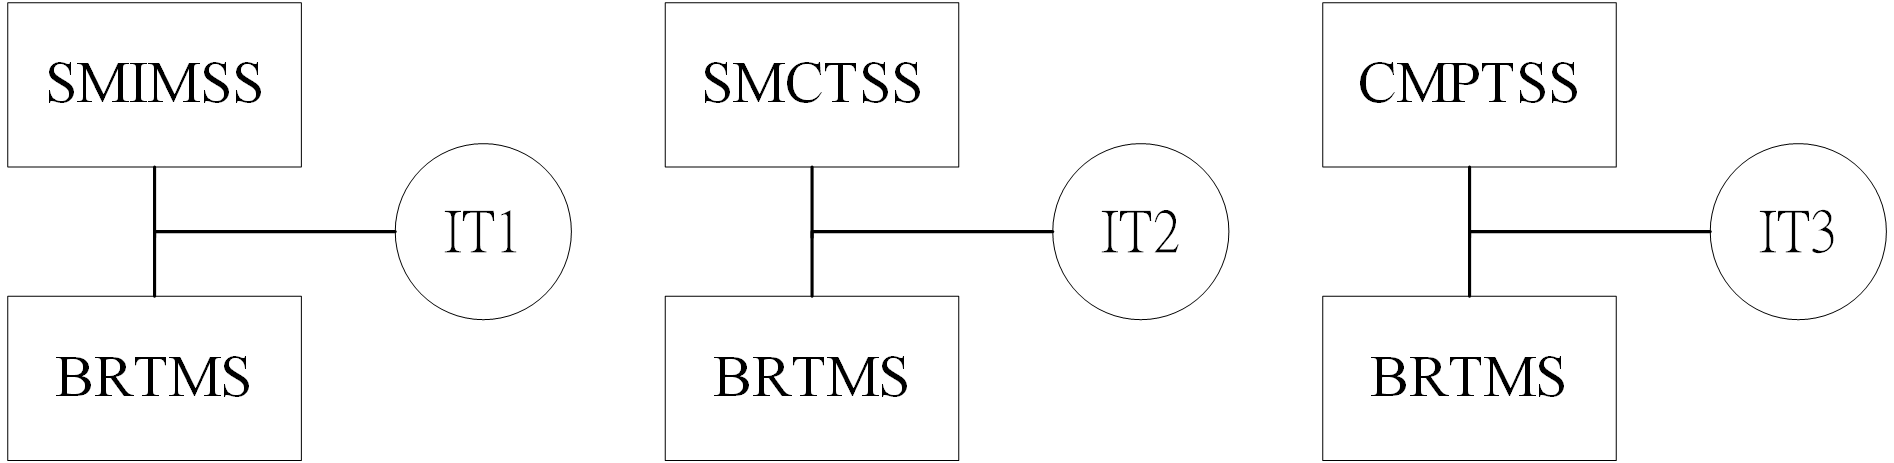
\includegraphics[width = 0.8\textwidth]{IntegrationTesting.png}
					\caption{集成子系统测试}\label{IntegrationTesting}
				\end{figure}
			\item 验收测试规划(Acceptance Testing,AT):
				本系统须达成以下三组接受用例陈列的所有功能,测试本论文设计与搭建的系统功能是否能够顺利运行。测试的角色有两个,分别为管理员以及用户,如图\ref{usecasediagram}为BTMS用例示意图,预计测试服务器的组态设置、手机的组态设置以及数据库的组态设置:

					\begin{figure}[!htbp]
						\centering
						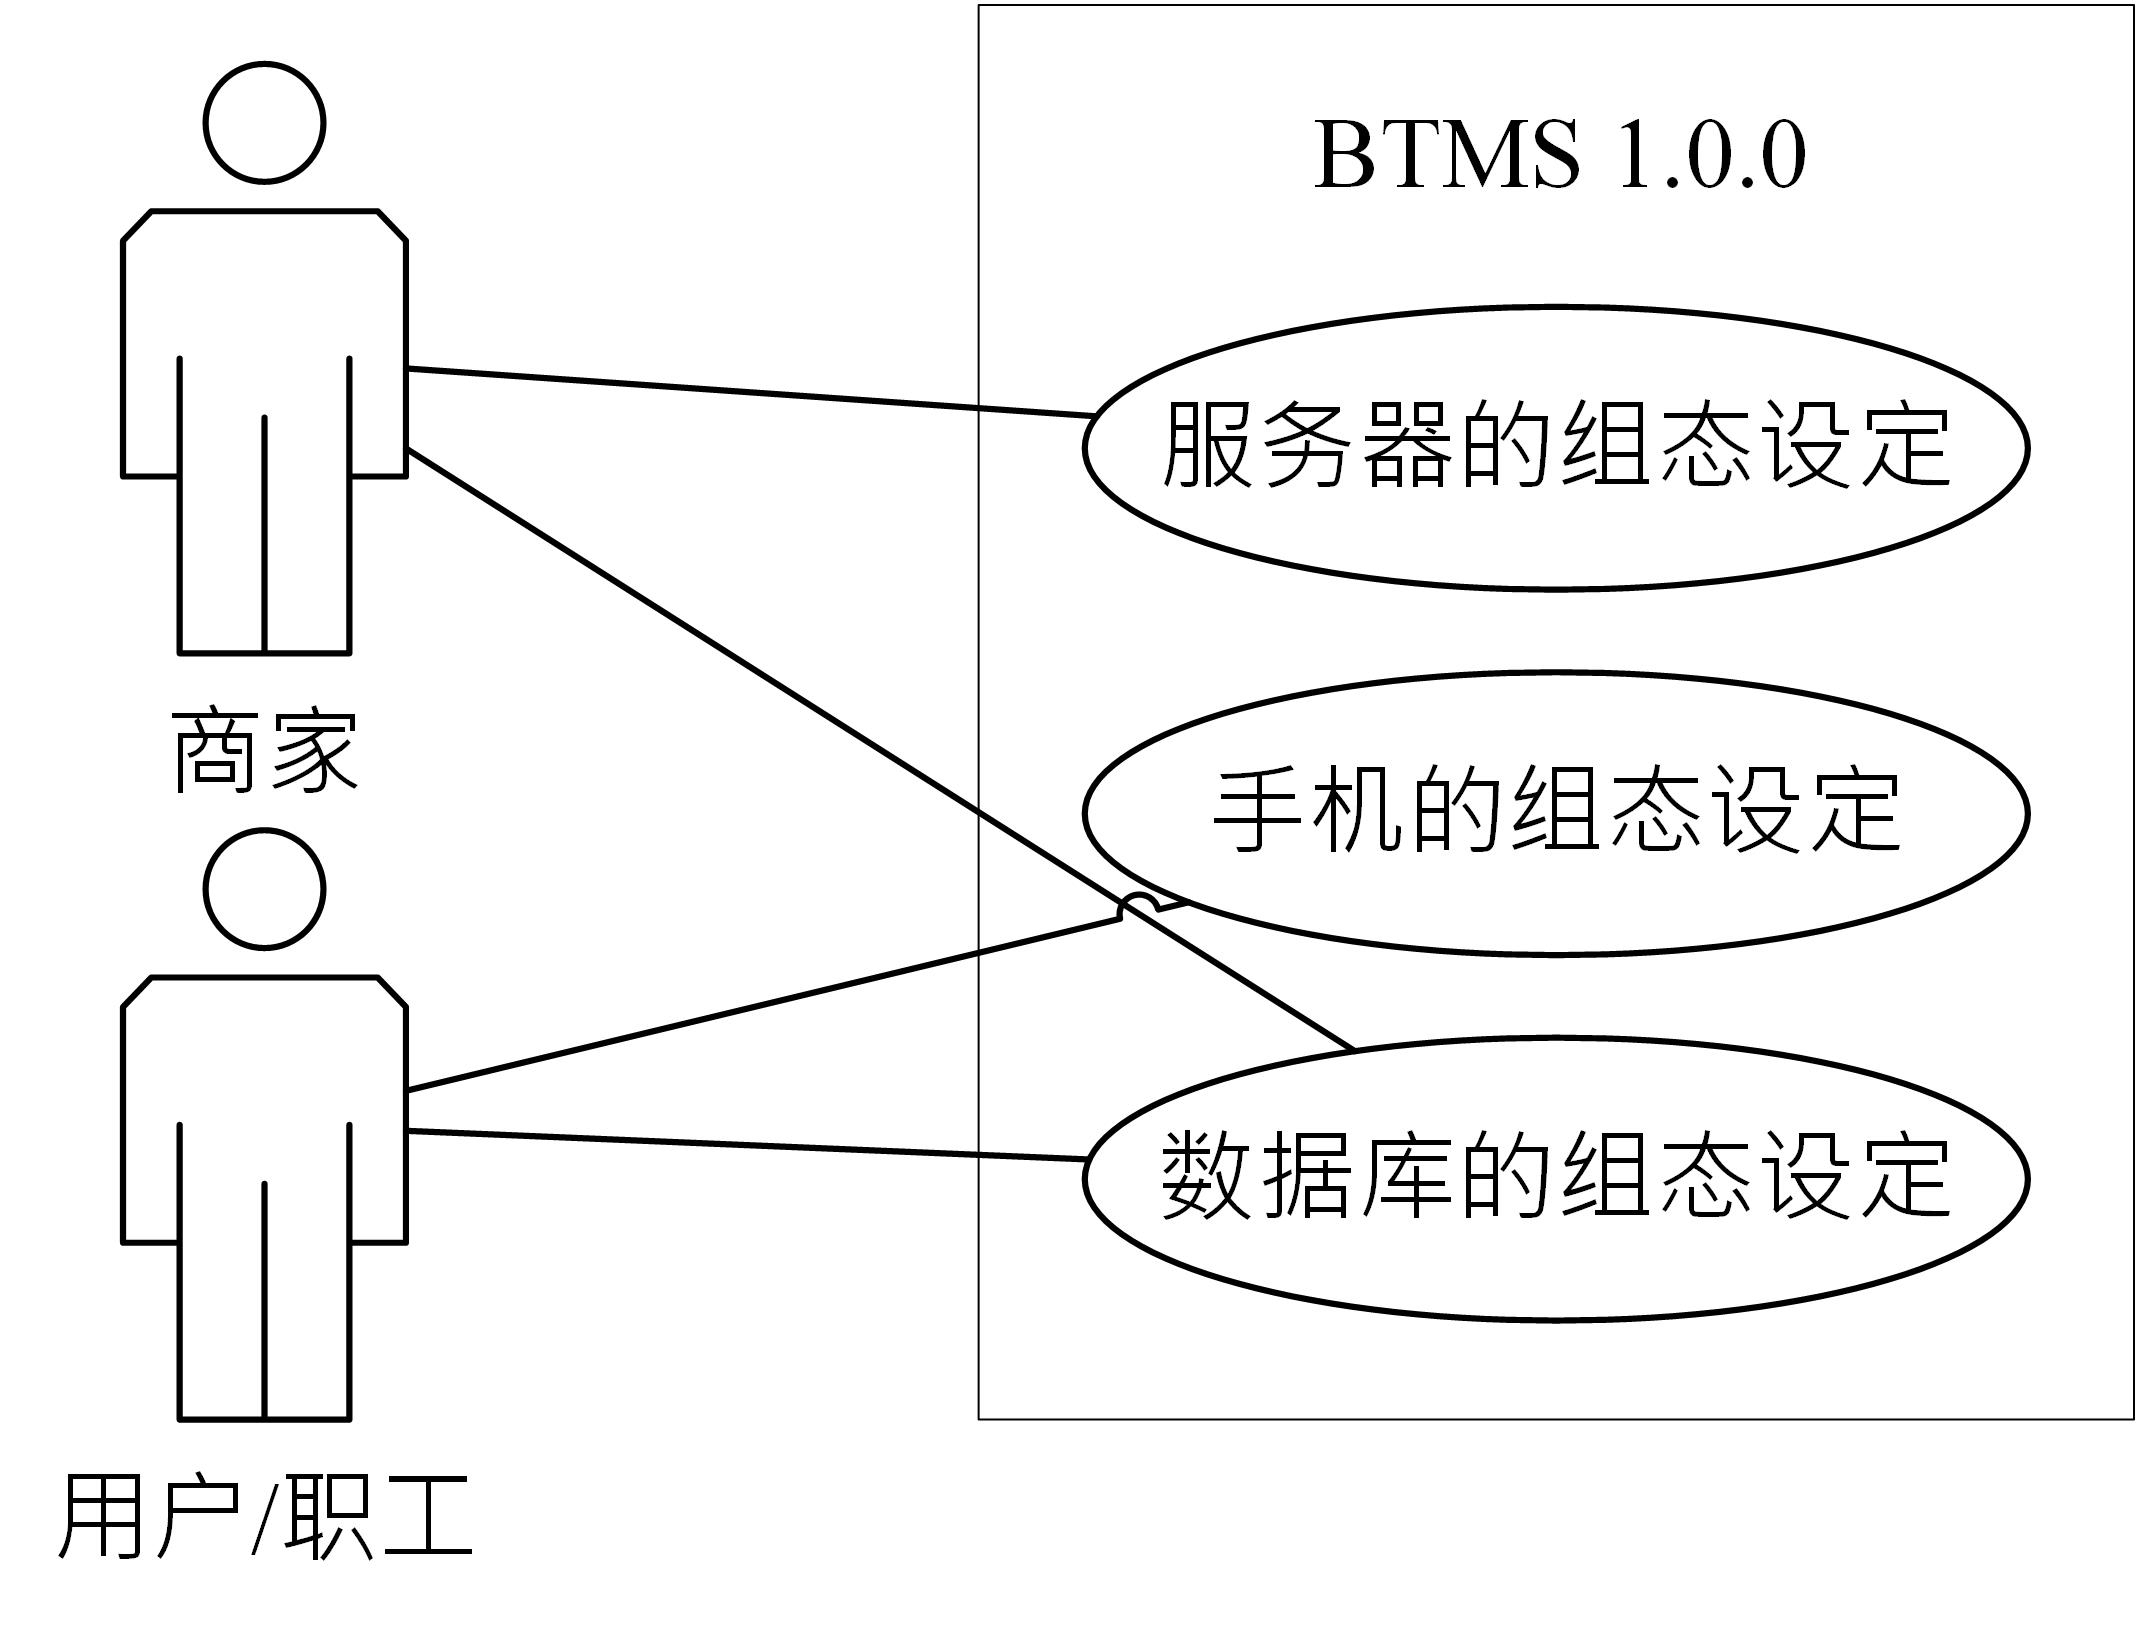
\includegraphics[width = 0.4\textwidth]{usecasediagram.jpg}
						\caption{BTMS用户用例图}\label{usecasediagram}
					\end{figure}

				图\ref{AcceptanceTesting}为三组验收测试的示意图,对本比特币的交易监督系统进行测试。
					\begin{figure}[!htbp]
						\centering
						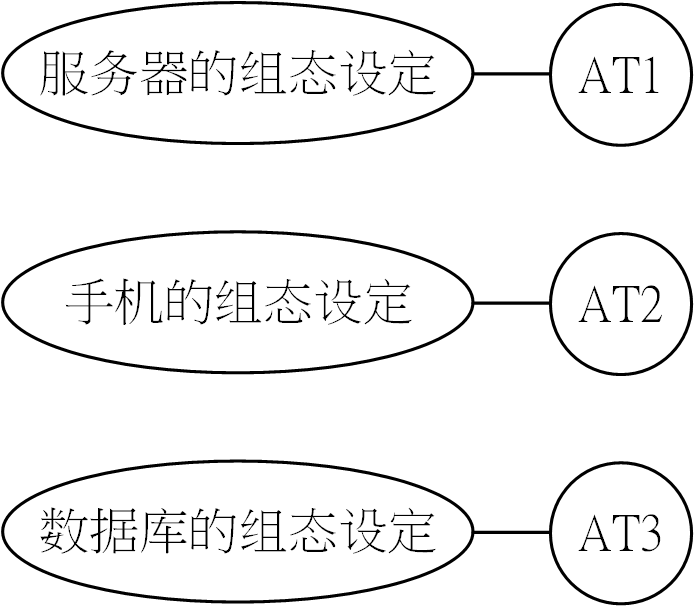
\includegraphics[width = 0.3\textwidth]{AcceptanceTesting.png}
						\caption{验收测试(Acceptance Testing)}\label{AcceptanceTesting}
					\end{figure}

	 		\end{enumerate}			

		\subsection{测试用例}
			\begin{enumerate}

			\item 集成测试(Integration Test):
				\begin{enumerate}

				\item IT1 测试用例:
					表\ref{IT1TestCase}为IT1 测试用例,测试对象为商家和商品信息管理子系统。目的:验证[SMIMSS 1.1.0]子系统能否正确管理商品信息。

					\begin{table}[!htbp]
					\centering
					\caption{IT1 测试用例}
					\label{IT1TestCase}
					\begin{tabular}{|l|l|}
					\hline
					用例ID & IT1 \\ \hline
					用例名称 & 集成SMIMSS至BTMS \\ \hline
					测试目标 & {[}SMIMSS 1.1.0{]}、{[}BTMS 1.0.0{]} \\ \hline
					依赖关系 & SMIMSS-F-001$\sim$ SMIMSS-F-005 \\ \hline
					严重程度 & 1(Critical) \\ \hline
					\multirow{5}{*}{用例描述} & 1.     能够添加店家帐户 \\ \cline{2-2} 
					 & 2.     能够添加/修改/删除店员帐户 \\ \cline{2-2} 
					 & 3.     能够添加/删除/修改商品信息 \\ \cline{2-2} 
					 & 4.     能够取得产品信息 \\ \cline{2-2} 
					 & 5.     能够接收交易信息 \\ \hline
					\multirow{5}{*}{预期结果} & 1.     成功添加店家帐户 \\ \cline{2-2} 
					 & 2.     成功添加/修改/删除店员帐户 \\ \cline{2-2} 
					 & 3.     成功添加/修改/删除商品信息 \\ \cline{2-2} 
					 & 4.     成功取得产品信息 \\ \cline{2-2} 
					 & 5.     成功接收交易信息 \\ \hline
					Cleanup & 无 \\ \hline
					\end{tabular}
					\end{table}


				\item IT2测试用例:
					表\ref{IT2TestCase}为IT2 测试用例目标,测试对象为商家手持移动装置收款及交易子系统。目的:验证[SMCTSS 1.2.0]子系统是否能够完成一笔行动支付之交易。

						\begin{table}[!htbp]
						\caption{IT2 测试用例} % title of Table
						\centering % used for centering table
						\label{IT2TestCase} % is used to refer this table in the text
						\begin{tabular}{|l|l|}
						\hline
						用例ID & IT2 \\ \hline
						用例名称 & 集成SMCTSS至BTMS \\ \hline
						测试目标 & {[}SMCTSS 1.2.0{]}、{[}BTMS 1.0.0{]} \\ \hline
						依赖关系 & SMCTSS-F-001$\sim$ SMCTSS-F-007 \\ \hline
						严重程度 & 1(Critical) \\ \hline
						\multirow{7}{*}{用例描述} & 1.     能够登入店员帐户 \\ \cline{2-2} 
						 & 2.     能够扫描NFC标签 \\ \cline{2-2} 
						 & 3.     能够读取商品信息 \\ \cline{2-2} 
						 & 4.     能够创建交易清单 \\ \cline{2-2} 
						 & 5.     能够发送交易信息 \\ \cline{2-2} 
						 & 6.     能够认证交易信息 \\ \cline{2-2} 
						 & 7.     能够存储交易明细 \\ \hline
						\multirow{7}{*}{预期结果} & 1.     成功登入店员帐户 \\ \cline{2-2} 
						 & 2.     成功扫描NFC标签 \\ \cline{2-2} 
						 & 3.     成功读取商品信息 \\ \cline{2-2} 
						 & 4.     成功创建交易清单 \\ \cline{2-2} 
						 & 5.     成功发送交易信息 \\ \cline{2-2} 
						 & 6.     成功认证交易信息 \\ \cline{2-2} 
						 & 7.     成功存储交易明细 \\ \hline
						Cleanup & 无 \\ \hline
						\end{tabular}
						\end{table}

				\item IT3测试用例:
					表\ref{IT3TestCase}为IT3 测试用例,目标测试对象为客户端行动支付和交易子系统。目的:验证[CMPTSS 1.3.0]能正确接收SMCTSS所发送的交易数据,并以其交易信息运行以比特币付款之动作。可以查找商品信息,且能够存储并且查看用户过往之交易纪录。

						\begin{table}[!htbp]
						\caption{IT3 测试用例} % title of Table
						\centering % used for centering table
						\label{IT3TestCase} % is used to refer this table in the text
						\begin{tabular}{|l|l|}
						\hline
						用例ID & IT3 \\ \hline
						用例名称 & 集成CMPTSS至BTMS \\ \hline
						测试目标 & {[}CMPTSS 1.3.0{]}、{[}BTMS 1.0.0{]} \\ \hline
						依赖关系 & CMPTSS-F-001$\sim$ CMPTSS-F-007 \\ \hline
						严重程度 & 1(Critical) \\ \hline
						\multirow{7}{*}{用例描述} & 1.     能够登入顾客帐号 \\ \cline{2-2} 
						 & 2.     能够读取商品信息 \\ \cline{2-2} 
						 & 3.     能够接收交易清单 \\ \cline{2-2} 
						 & 4.     能够认证交易信息 \\ \cline{2-2} 
						 & 5.     能够运行行动支付 \\ \cline{2-2} 
						 & 6.     能够存储交易明细 \\ \cline{2-2} 
						 & 7.     能够查看交易纪录 \\ \hline
						\multirow{7}{*}{预期结果} & 1.     成功登入顾客帐号 \\ \cline{2-2} 
						 & 2.     成功读取商品信息 \\ \cline{2-2} 
						 & 3.     成功接收交易清单 \\ \cline{2-2} 
						 & 4.     成功认证交易信息 \\ \cline{2-2} 
						 & 5.     成功运行行动支付 \\ \cline{2-2} 
						 & 6.     成功存储交易纪录 \\ \cline{2-2} 
						 & 7.     成功查看交易纪录 \\ \hline
						Cleanup & 无 \\ \hline
						\end{tabular}
						\end{table}
				\end{enumerate}

		\item 验收测试用例(Acceptance Testing Cases):
			验收测试用例目的在于测试母系统BTMS、子系统SMIMSS、SMCTSS与CMPTSS是否能够顺利的进行信息传递完成交互。

			\begin{enumerate}
				\item AT1 测试用例:
					表\ref{AT1TestCase}所示,目标测试管理人员是否能够顺利使用子系统SMIMSS顺利与母系统BTMS交互。目的:验证使用用例(Use case)1,透过组态文件的修改对服务器进行组态设置。

						\begin{table}[!htbp]
						\centering
						\caption{AT1 测试用例}
						\label{AT1TestCase}
						\begin{tabular}{|l|l|l|}
						\hline
						用例ID & \multicolumn{2}{l|}{AT1} \\ \hline
						用例名称 & \multicolumn{2}{l|}{服务器的组态设置} \\ \hline
						测试目标 & \multicolumn{2}{l|}{\begin{tabular}[c]{@{}l@{}}{[}SMIMSS 1.1.0{]}\\ {[}BTMS 1.0.0{]}\end{tabular}} \\ \hline
						依赖关系 & \multicolumn{2}{l|}{BTMS-F-001} \\ \hline
						严重程度 & \multicolumn{2}{l|}{1(Critical)} \\ \hline
						\multirow{3}{*}{用例描述} & 用户操作 & 系统响应 \\ \cline{2-3} 
						 & \begin{tabular}[c]{@{}l@{}}1.管理人员依照环境\\    设置服务器组态。\end{tabular} &  \\ \cline{2-3} 
						 &  & \begin{tabular}[c]{@{}l@{}}2.服务器依照管理人\\    员所做的组态设置\\    启动服务。\end{tabular} \\ \hline
						预期结果 & \multicolumn{2}{l|}{成功启动服务器的相关服务。} \\ \hline
						Cleanup & \multicolumn{2}{l|}{无} \\ \hline
						\end{tabular}
						\end{table}

				\item AT2 测试用例:
					如表\ref{AT2TestCase}所示,参与者为用户。目的:验证用例(Use case )2 透过组态文件的修改对手机进行组态设置。
						\begin{table}[!htbp]
						\centering
						\caption{AT2 测试用例}
						\label{AT2TestCase}
						\begin{tabular}{|l|l|l|}
						\hline
						用例ID & \multicolumn{2}{l|}{AT2} \\ \hline
						用例名称 & \multicolumn{2}{l|}{手机的组态设置} \\ \hline
						测试目标 & \multicolumn{2}{l|}{\begin{tabular}[c]{@{}l@{}}{[}SMCTSS 1.2.0{]}\\ {[}CMPTSS 1.3.0{]}\end{tabular}} \\ \hline
						依赖关系 & \multicolumn{2}{l|}{BTMS-F-002$\sim$ BTMS-F-003} \\ \hline
						严重程度 & \multicolumn{2}{l|}{1(Critical)} \\ \hline
						\multirow{3}{*}{用例描述} & 用户操作 & 系统响应 \\ \cline{2-3} 
						 & \begin{tabular}[c]{@{}l@{}}1.用户修改手机组\\    态设置参数。\end{tabular} &  \\ \cline{2-3} 
						 &  & \begin{tabular}[c]{@{}l@{}}2.手机依照用户在\\    设置档中所填入的\\    数值运作。\end{tabular} \\ \hline
						预期结果 & \multicolumn{2}{l|}{成功完成手机的组态设置} \\ \hline
						Cleanup & \multicolumn{2}{l|}{无} \\ \hline
						\end{tabular}
						\end{table}

				\item AT3 测试用例:
					如表\ref{AT3TestCase}所示,目的:验证用例(Use case )3,透过组态文件的修改对数据库进行组态设置。

						\begin{table}[!htbp]
						\centering
						\caption{AT3 测试用例}
						\label{AT3TestCase}
						\begin{tabular}{|l|l|l|}
						\hline
						用例ID & \multicolumn{2}{l|}{AT3} \\ \hline
						用例名称 & \multicolumn{2}{l|}{数据库的组态设置} \\ \hline
						测试目标 & \multicolumn{2}{l|}{\begin{tabular}[c]{@{}l@{}}{[}SMIMSS 1.1.0{]}\\ {[}SMCTSS 1.2.0{]}\\ {[}CMPTSS 1.3.0{]}\end{tabular}} \\ \hline
						依赖关系 & \multicolumn{2}{l|}{BTMS-F-001$\sim$ BTMS-F-003} \\ \hline
						严重程度 & \multicolumn{2}{l|}{1(Critical)} \\ \hline
						\multirow{5}{*}{用例描述} & 用户操作 & 系统响应 \\ \cline{2-3} 
						 & \begin{tabular}[c]{@{}l@{}}1.管理者设置数据库\\    组态。\end{tabular} &  \\ \cline{2-3} 
						 &  & \begin{tabular}[c]{@{}l@{}}2.数据库依照管理人\\    员所做的组态设置\\    启动服务。\end{tabular} \\ \cline{2-3} 
						 & \begin{tabular}[c]{@{}l@{}}3.用户修改数据库\\    之数据及文件。\end{tabular} &  \\ \cline{2-3} 
						 &  & \begin{tabular}[c]{@{}l@{}}4.数据库依照用户\\    所做的组态设置启\\    动服务。\end{tabular} \\ \hline
						预期结果 & \multicolumn{2}{l|}{成功设置完成数据库的相关设置。} \\ \hline
						Cleanup & \multicolumn{2}{l|}{无} \\ \hline
						\end{tabular}
						\end{table}
			\end{enumerate}
		\end{enumerate}

		\subsection{测试结果和分析}
		\begin{enumerate}

			\item 集成测试用例(Integration Testing Cases)
			表\ref{table8}为IT1、为IT2、为IT3的集成子系统测试结果,皆顺利运作。

				\begin{table}[!htbp]
				\centering
				\caption{集成子系统测试结果}
				\label{table8}
				\begin{tabular}{|c|c|l|}
				\hline
				测试用例 & 结果 (通过/不通过) & Comment \\ \hline
				\multirow{5}{*}{IT1} & \multirow{5}{*}{通过} & 1.成功添加店家帐户 \\ \cline{3-3} 
				 &  & 2.成功添加/修改/删除店员帐户 \\ \cline{3-3} 
				 &  & 3.成功添加/修改/删除商品信息 \\ \cline{3-3} 
				 &  & 4.成功取得产品信息 \\ \cline{3-3} 
				 &  & 5.成功接收交易信息 \\ \hline
				\multirow{7}{*}{IT2} & \multirow{7}{*}{通过} & 1.成功登入店员帐户 \\ \cline{3-3} 
				 &  & 2.成功扫描NFC标签 \\ \cline{3-3} 
				 &  & 3.成功读取商品信息 \\ \cline{3-3} 
				 &  & 4.成功创建交易清单 \\ \cline{3-3} 
				 &  & 5.成功发送交易信息 \\ \cline{3-3} 
				 &  & 6.成功认证交易信息 \\ \cline{3-3} 
				 &  & 7.成功存储交易明细 \\ \hline
				\multirow{7}{*}{IT3} & \multirow{7}{*}{通过} & 1.成功登入顾客帐号 \\ \cline{3-3} 
				 &  & 2.成功读取商品信息 \\ \cline{3-3} 
				 &  & 3.成功接收交易清单 \\ \cline{3-3} 
				 &  & 4.成功认证交易信息 \\ \cline{3-3} 
				 &  & 5. 成功运行行动支付 \\ \cline{3-3} 
				 &  & 6.成功存储交易纪录 \\ \cline{3-3} 
				 &  & 7.成功查看交易纪录 \\ \hline
				RATE & 90\% & \begin{tabular}[c]{@{}l@{}}BTMS开发透过手机让商家及顾客\\ 以手机发送交易信息,如:商品\\ 名称、商品金额,商家收款地址。\\ 并且及时将商品信息更新至服务器\\ 之数据库,以便商家控管商品信息\\ 状态,同时让顾客可以享受数字加\\ 密货币的方便性。\end{tabular} \\ \hline
				\end{tabular}
				\end{table}

			\item 验收测试用例(Acceptance Testing Cases)
			表\ref{table9}为前节所设计的三种AT1、AT2与AT3的验收测试结果,皆顺利运行。
				\begin{table}[!htbp]
				\centering
				\caption{验收测试结果}
				\label{table9}
				\begin{tabular}{|c|c|l|}
				\hline
				测试用例 & 结果(通过/不通过) & Comment \\ \hline
				AT1 & 通过 & 成功启动服务器的相关服务。 \\ \hline
				AT2 & 通过 & 成功完成手机的组态设置。 \\ \hline
				AT3 & 通过 & 成功设置完成数据库的相关设置。 \\ \hline
				RATE & 100\% & \begin{tabular}[c]{@{}l@{}}BTMS可透过组态设置的方式来设\\ 定各个子系统的环境参数。\end{tabular} \\ \hline
				\end{tabular}
				\end{table}
						\begin{table}[!htbp]
						\centering
						\caption{子系统与测试用例关系表}
						\label{table10}
						\begin{tabular}{|l|c|c|c|}
						\hline
						 & \multicolumn{1}{l|}{SMIMSS 1.1.0} & \multicolumn{1}{l|}{SMCTSS 1.2.0} & \multicolumn{1}{l|}{CMPISS 1.3.0} \\ \hline
						IT1 & X &  &  \\ \hline
						IT2 &  & X &  \\ \hline
						IT3 &  &  & X \\ \hline
						AT1 & X &  &  \\ \hline
						AT2 &  & X & X \\ \hline
						AT3 & X & X & X \\ \hline
						\end{tabular}
						\end{table}

						\begin{table}[!htbp]
					\centering
					\caption{需求与集成测试用例的关系表}
					\label{table11}
					\begin{tabular}{|l|c|c|c|}
					\hline
					 & \multicolumn{1}{l|}{IT1} & \multicolumn{1}{l|}{IT2} & \multicolumn{1}{l|}{IT3} \\ \hline
					BTMS-F-001 & X &  &  \\ \hline
					BTMS-F-002 &  & X &  \\ \hline
					BTMS-F-003 &  &  & X \\ \hline
					SMIMSS-F-001 & X &  &  \\ \hline
					SMIMSS-F-002 & X &  &  \\ \hline
					SMIMSS-F-003 & X &  &  \\ \hline
					SMIMSS-F-004 & X &  &  \\ \hline
					SMIMSS-F-005 & X &  &  \\ \hline
					SMCTSS-F-001 &  & X &  \\ \hline
					SMCTSS-F-002 &  & X &  \\ \hline
					SMCTSS-F-003 &  & X &  \\ \hline
					SMCTSS-F-004 &  & X &  \\ \hline
					SMCTSS-F-005 &  & X &  \\ \hline
					SMCTSS-F-006 &  & X &  \\ \hline
					SMCTSS-F-007 &  & X &  \\ \hline
					CMPTSS-F-001 &  &  & X \\ \hline
					CMPTSS-F-002 &  &  & X \\ \hline
					CMPTSS-F-003 & \multicolumn{1}{l|}{} & \multicolumn{1}{l|}{} & X \\ \hline
					CMPTSS-F-004 & \multicolumn{1}{l|}{} & \multicolumn{1}{l|}{} & X \\ \hline
					CMPTSS-F-005 & \multicolumn{1}{l|}{} & \multicolumn{1}{l|}{} & X \\ \hline
					CMPTSS-F-006 & \multicolumn{1}{l|}{} & \multicolumn{1}{l|}{} & X \\ \hline
					CMPTSS-F-007 & \multicolumn{1}{l|}{} & \multicolumn{1}{l|}{} & X \\ \hline
					\end{tabular}
					\end{table}


					\begin{table}[!htbp]
					\centering
					\caption{需求与验收测试案例的关系表}
					\label{table12}
					\begin{tabular}{|l|c|c|c|}
					\hline
					 & \multicolumn{1}{l|}{AT1} & \multicolumn{1}{l|}{AT2} & \multicolumn{1}{l|}{AT3} \\ \hline
					BTMS-F-001 & X &  & X \\ \hline
					BTMS-F-002 &  & X & X \\ \hline
					BTMS-F-003 &  & X & X \\ \hline
					\end{tabular}
					\end{table}


			\item 可追踪性(Traceability)

						

			\begin{enumerate}
				\item 子系统与测试用例:表\ref{table10}为测试组IT1、IT2、IT3、AT1、AT2、AT3与子系统SMIMSS、SMCTSS、CMPISS的关系表。
				\item 需求与测试用例:表\ref{table11}为本系统需求与集成测试用例的关系表,表\ref{table12}为需求与验收测试案例的关系表。
				\end{enumerate}
		\end{enumerate}


	\section{性能测试}


		\begin{figure}[!htbp]
			\centering
			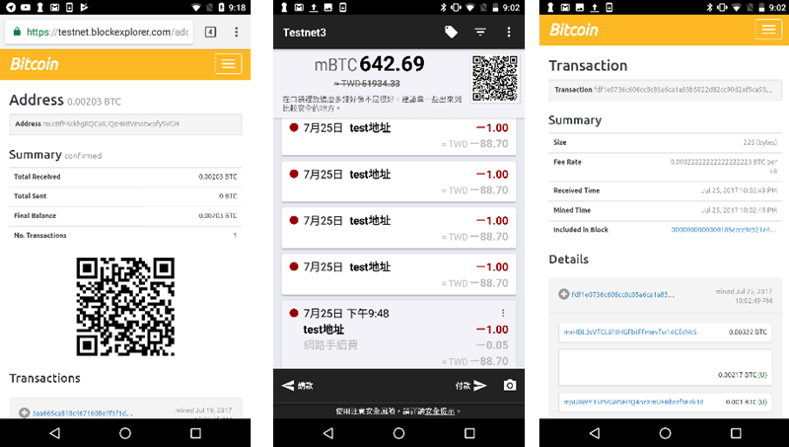
\includegraphics[width = 0.8\textwidth]{fig9.png}
			\caption{使用区块链查看器验证存储在比特币区块链中的交易过程}\label{fig9}
		\end{figure}


		根据比特币点对点架构,尽管顾客和商家之间的交易细节已经快速存储到云数据库,但官方确认交易与当前比特币区块链的交易通常需要更长的时间,因为需要确保确认的数量在交易广播比特币点对点网络并存储到缓存池后,是否存在双重支付。本文设计了比特币的交易监督系统以及引用多重签章算法重新设计的比特币的实时交易监督系统,以下将分别针对有无采用多重签章算法的性能测试。


		\subsection{系统性能测试}
		为了验证本文提出的BTMS不会通过使用比特币等加密货币影响交易完成时间,于2017年7月25日、2017年9月6日以及2018年3月21日,在Testnet实验中连续记录了20笔交易信息,每1秒发出一笔交易,分别历时20分钟。

		\begin{enumerate}
			\item 初始测试(2017年7月25日):
			首先,使用区块链查看器(Blockchain Explorer)\supercite{Blockchainexplorer:Ananalyticalprocessandinvestigationenvironmentforbitcoin},如\ref{fig9}的快照所示,透过使用Testnet依序进行20笔比特币交易,如图\ref{fig9}的中间快照所示,最后20笔交易完成时间全部记录在区块链查看器。实验结果显示,实验中的所有交易都在3秒钟左右(平均2.97秒,标准差小于1秒)发送到比特币网络缓存池,平均交易完成时间在比特币区块链中确认为522.33秒(小于9分钟),标准差大约为339秒。

			\item 第一次测试(2017年9月6日):表\ref{1general}为第一次实验数据,该次的比特币交易发起广播至比特币交易缓存池的时间平均为1.918秒,标准差为0.55586秒。但为了预防双重支付攻击需要等待平均654.8秒(小于11分钟,标准差346.63秒)的时间。

				\begin{table}[!htbp]
				\centering
				\caption{第一次Testnet 运行实验之数据分析(2017年9月6日)}
				\label{1general}
				\begin{tabular}{|c|c|c|c|}
				\hline
				         & 进入缓存池时间(秒) & 进入区块链时间(秒)    & 完成交易时间(秒)     \\ \hline
				平均       & 1.918      & 654.8         & 654.8         \\ \hline
				样本标准差    & 0.55586    & 346.63        & 346.63        \\ \hline
				95\%信赖区间 & 1.69~2.15  & 511.72~797.88 & 511.72~797.88 \\ \hline
				99\%信赖区间 & 1.61~2.23  & 460.9~848.7   & 460.9~848.7   \\ \hline
				\end{tabular}
				\end{table}

			\item 第二次测试(2018年3月21日):表\ref{2general}为第二次测试的实验原始数据,表\ref{2general-1}为将数据进行分析后的结果可以看出,平均进入缓存池的时间为1.12秒,进入区块链的时间为287.12秒,因为并未采用多重签章算法,所以交易完成时间以287.12秒计算。
				\begin{table}[!htbp]
				\centering
				\caption{第二次Testnet 运行实验数据(2018年3月21日)}
				\label{2general}
				\begin{tabular}{|c|c|c|c|c|c|}
				\hline
				\begin{tabular}[c]{@{}c@{}}交易\\ 次数\end{tabular} & 付款时间 & \begin{tabular}[c]{@{}c@{}}进入缓存池\\ 所花时间(秒)\end{tabular} & \begin{tabular}[c]{@{}c@{}}进入缓存池\\ 时间点\end{tabular} & \begin{tabular}[c]{@{}c@{}}写入区块链\\ 所花时间(秒)\end{tabular} & \begin{tabular}[c]{@{}c@{}}写入区块\\ 时间点\end{tabular} \\ \hline
				1 & 0:00:00 & 3 & 0:00:03 & 136 & 0:02:16 \\ \hline
				2 & 0:01:00 & 1 & 0:01:01 & 76 & 0:02:16 \\ \hline
				3 & 0:02:04 & 3 & 0:02:07 & 12 & 0:02:16 \\ \hline
				4 & 0:03:00 & 1 & 0:03:01 & 438 & 0:10:18 \\ \hline
				5 & 0:04:00 & 1 & 0:04:01 & 378 & 0:10:18 \\ \hline
				6 & 0:05:00 & 1 & 0:05:01 & 318 & 0:10:18 \\ \hline
				7 & 0:06:00 & 2 & 0:06:02 & 258 & 0:10:18 \\ \hline
				8 & 0:07:00 & 1 & 0:07:01 & 198 & 0:10:18 \\ \hline
				9 & 0:08:00 & 1 & 0:08:01 & 138 & 0:10:18 \\ \hline
				10 & 0:09:00 & 1 & 0:09:01 & 78 & 0:10:18 \\ \hline
				11 & 0:10:00 & 1 & 0:10:01 & 18 & 0:10:18 \\ \hline
				12 & 0:11:00 & 2 & 0:11:02 & 810 & 0:24:30 \\ \hline
				13 & 0:12:00 & 1 & 0:12:01 & 750 & 0:24:30 \\ \hline
				14 & 0:13:00 & 1 & 0:13:01 & 690 & 0:24:30 \\ \hline
				15 & 0:14:00 & 1 & 0:14:01 & 630 & 0:24:30 \\ \hline
				16 & 0:15:00 & 1 & 0:15:01 & 570 & 0:24:30 \\ \hline
				17 & 0:16:00 & 2 & 0:16:02 & 510 & 0:24:30 \\ \hline
				18 & 0:17:00 & 2 & 0:17:02 & 450 & 0:24:30 \\ \hline
				19 & 0:18:00 & 1 & 0:18:01 & 390 & 0:24:30 \\ \hline
				20 & 0:19:00 & 1 & 0:19:01 & 330 & 0:24:30 \\ \hline
				\end{tabular}
				\end{table}

				\begin{table}[!htbp]
				\centering
				\caption{第二次以Testnet 运行实验数据分析(2018年3月21日)}
				\label{2general-1}
				\begin{tabular}{|c|c|c|c|}
				\hline
				         & 进入缓存池时间(秒) & 进入区块链时间(秒)    & 完成交易时间(秒)     \\ \hline
				平均       & 1.12       & 287.12        & 287.12        \\ \hline
				样本标准差    & 0.68       & 246.59        & 246.59        \\ \hline
				95\%信赖区间 & 0.84~1.4   & 185.33~388.91 & 185.33~388.91 \\ \hline
				99\%信赖区间 & 0.74~1.5   & 149.18~425.06 & 149.18~425.06 \\ \hline
				\end{tabular}
				\end{table}


		\end{enumerate}

			在未引用多重签章算法的监督系统中,第一次与第二次的测试相比并无太大的差异,交易完成时间与比特币区块生成所需时间相同,平均时间皆为十分钟。根据比特币Testnet上的初步实验结果显示,本文提出的BTMS可以快速有效地运行比特币的交易监督系统。

			%

		\subsection{实时系统性能测试}
		本节介绍比特币测试币于Government Green Address钱包进行交易的性能实验与结果分析,包含该实验的目的、方法及结果分析。实验的目的是要确认的系统在商家端进行行动支付时能快速、精准且高效率的进行交易,并了解使用一般Testnet钱包与Government Green Address钱包作为交易媒介的确认交易时间的差距。表\ref{0test}为2017年7月25日初步的采用多重签章算法的测试数据,数据显示交易存储到区块链的平均时间为10分钟,但Government Green Address采用的多重签章算法,可以有效拒绝双重花费的交易发起,因此可将交易的有效时间,从交易进入区块链的时间,重新订定为交易进入比特币交易缓存池的时间。

		\begin{table}[!htbp]
			\centering
			\caption{初步的Government Green Address实验测试数据 (2017年7月25日)}
			\label{0test}
			\begin{tabular}{|c|c|c|c|c|}
			\hline
			\multicolumn{1}{|c|}{付款时间} & \multicolumn{1}{c|}{\begin{tabular}[c]{@{}c@{}}进入缓存池\\ 所花时间(秒)\end{tabular}} & \multicolumn{1}{c|}{\begin{tabular}[c]{@{}c@{}}进入缓存池\\ 时间点\end{tabular}} & \multicolumn{1}{c|}{入块时间} & \multicolumn{1}{c|}{\begin{tabular}[c]{@{}c@{}}写入区块\\ 费时间\end{tabular}} \\ \hline
			06:36:25 & 2.14 & 06:36:27.14 & 06:52:00 & 16:25 \\ \hline
			06:38:25 & 1.075 & 06:38:26.075 & 06:52:00 & 14:25 \\ \hline
			06:40:25 & 1.722 & 06:40:26.722 & 06:52:00 & 12:25 \\ \hline
			06:42:25 & 2.953 & 06:42:27.953 & 06:52:00 & 10:25 \\ \hline
			06:44:25 & 1.511 & 06:44:26.511 & 06:52:00 & 08:25 \\ \hline
			06:46:25 & 2.269 & 06:46:27.269 & 06:52:00 & 06:25 \\ \hline
			06:48:25 & 1.831 & 06:48:26.831 & 06:52:00 & 04:25 \\ \hline
			06:50:25 & 1.227 & 06:50:26.227 & 06:52:00 & 02:25 \\ \hline
			06:52:25 & 2.026 & 06:52:27.026 & 07:12:01 & 20:24 \\ \hline
			06:54:25 & 1.257 & 06:54:26.257 & 07:12:01 & 18:24 \\ \hline
			06:56:25 & 1.511 & 06:56:26.511 & 07:12:01 & 16:24 \\ \hline
			06:58:25 & 2.815 & 06:58:27.815 & 07:12:01 & 14:24 \\ \hline
			07:00:26 & 1.544 & 07:00:27.544 & 07:12:01 & 12:25 \\ \hline
			07:02:25 & 1.767 & 07:02:26.767 & 07:12:01 & 10:24 \\ \hline
			07:04:25 & 1.52 & 07:04:26.52 & 07:12:01 & 08:24 \\ \hline
			07:06:25 & 1.953 & 07:06:26.953 & 07:12:01 & 06:24 \\ \hline
			\end{tabular}
			\end{table}


		本次的实验分为两部份,分别是透过比特币 Testnet钱包以及使用本论文所采用的Government Green Address比特币钱包上运行20次付款,皆以相同地址收款,交易金额都设置为0.00001 BTC,实验时间为2017年9月6日与2018年2月6日,每隔一分钟运行一次付款的动作,总共历时20分钟。两款钱包同时发起交易,并透过区块链查看器进行记录时间,最后再比较使用一般比特币钱包及Government Green Address钱包两者之间的差距。

		\begin{enumerate}
			\item 第一次测试(2017年9月6日):表\ref{1green}为第一次测试实验的数据分析结果,平均进入交易缓存池的时间为2.11秒,真正写入区块链的时间为654.24秒,采用多重签章算法,这些交易不存在双重支付的问题,因此完成时间记为2.11秒。

			\begin{table}[!htbp]
				\centering
				\caption{第一次以Government Green Address运行实验之数据分析(2017年9月6日)}
				\label{1green}
				\begin{tabular}{|c|c|c|c|}
				\hline
				         & 进入缓存池时间(秒) & 进入区块链时间(秒)    & 完成交易时间(秒) \\ \hline
				平均       & 2.11       & 654.24        & 2.11      \\ \hline
				样本标准差    & 0.65       & 346.9         & 0.65      \\ \hline
				95\%信赖区间 & 1.84~2.38  & 511.05~797.43 & 1.84~2.38 \\ \hline
				99\%信赖区间 & 1.75~2.47  & 460.19~848.29 & 1.75~2.47 \\ \hline
				\end{tabular}
				\end{table}

			\item 第二次测试(2018年3月21日):表\ref{2green}为第二次以Government Green Address运行实验数据,表\ref{2green-1}为基于第二次测试的数据分析结果,进入缓存池的平均时间为1.55秒,进入区块链的平均时间为431.4秒,因为采用多重签章算法将完成交易时间以1.55秒计算。

		\end{enumerate}
			\begin{table}[!htbp]
				\centering
				\caption{第二次以Government Green Address运行实验数据(2018年3月21日)}
				\label{2green}
				\begin{tabular}{|c|c|c|c|c|c|}
				\hline
				\begin{tabular}[c]{@{}c@{}}交易\\ 次数\end{tabular} & 付款时间 & \begin{tabular}[c]{@{}c@{}}进入缓存池\\ 所花时间(秒)\end{tabular} & \begin{tabular}[c]{@{}c@{}}进入缓存池\\ 时间点\end{tabular} & \begin{tabular}[c]{@{}c@{}}写入区块链\\ 所花时间(秒)\end{tabular} & \begin{tabular}[c]{@{}c@{}}写入区块\\ 时间点\end{tabular} \\ \hline
				1 & 0:00:01 & 2 & 0:00:03 & 619 & 0:10:18 \\ \hline
				2 & 0:01:00 & 1 & 0:01:01 & 559 & 0:10:18 \\ \hline
				3 & 0:02:02 & 2 & 0:02:04 & 496 & 0:10:18 \\ \hline
				4 & 0:03:00 & 1 & 0:03:01 & 438 & 0:10:18 \\ \hline
				5 & 0:04:00 & 1 & 0:04:01 & 378 & 0:10:18 \\ \hline
				6 & 0:05:00 & 2 & 0:05:02 & 318 & 0:10:18 \\ \hline
				7 & 0:06:00 & 1 & 0:06:01 & 258 & 0:10:18 \\ \hline
				8 & 0:07:00 & 1 & 0:07:01 & 198 & 0:10:18 \\ \hline
				9 & 0:08:00 & 2 & 0:08:02 & 138 & 0:10:18 \\ \hline
				10 & 0:09:00 & 2 & 0:09:02 & 78 & 0:10:18 \\ \hline
				11 & 0:10:00 & 1 & 0:10:01 & 18 & 0:10:18 \\ \hline
				12 & 0:11:00 & 2 & 0:11:02 & 810 & 0:24:30 \\ \hline
				13 & 0:12:00 & 2 & 0:12:02 & 750 & 0:24:30 \\ \hline
				14 & 0:13:00 & 1 & 0:13:01 & 690 & 0:24:30 \\ \hline
				15 & 0:14:00 & 2 & 0:14:02 & 630 & 0:24:30 \\ \hline
				16 & 0:15:00 & 1 & 0:15:01 & 570 & 0:24:30 \\ \hline
				17 & 0:16:00 & 2 & 0:16:02 & 510 & 0:24:30 \\ \hline
				18 & 0:17:00 & 2 & 0:17:02 & 450 & 0:24:30 \\ \hline
				19 & 0:18:00 & 1 & 0:18:01 & 390 & 0:24:30 \\ \hline
				20 & 0:19:00 & 2 & 0:19:02 & 330 & 0:24:30 \\ \hline
				\end{tabular}
				\end{table}

			\begin{table}[!htbp]
				\centering
				\caption{第二次以Government Green Address运行实验之数据分析(2018年3月21日)}
				\label{2green-1}
				\begin{tabular}{|c|c|c|c|}
				\hline
				         & 进入缓存池时间(秒)     & 进入区块链时间(秒)         & 完成交易时间(秒)      \\ \hline
				平均       & 1.55           & 431.4              & 1.55           \\ \hline
				样本标准差    & 0.51           & 220.84             & 0.51           \\ \hline
				95\%信赖区间 & 1.34$\sim$1.76 & 340.24$\sim$522.56 & 1.34$\sim$1.76 \\ \hline
				99\%信赖区间 & 1.26$\sim$1.84 & 307.86$\sim$554.94 & 1.26$\sim$1.84 \\ \hline
				\end{tabular}
				\end{table}

				

				
				

	%			\begin{figure}[!htbp]
	%				\centering
	%				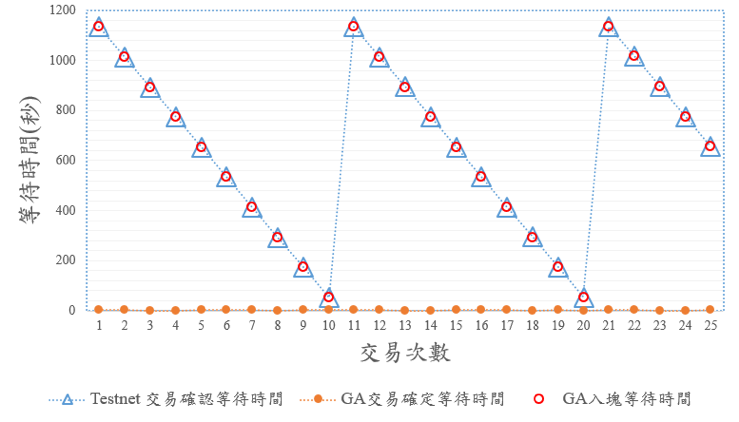
\includegraphics[width = 0.7\textwidth]{fig12.png}
	%				\caption{fig12}\label{fig12}
	%

%				\end{figure}

	本次实验分别记录以Testnet钱包及Government Green Address钱包运行20次交易的进入缓存池等待时间和写入区块等待时间。若以Testnet钱包交易,必须等到交易写入才能保证此笔交易不会被矿工遗弃,也才算真的完成这笔交易;但若以Government Green Address钱包发起交易就大不相同,当交易进入缓存池,即使遇到交易被矿工遗弃的情况,Government Green Address机构节点也会重新发起此笔交易,保证让交易写入区块,所以只要进入缓存池就可以视为交易完成,透过两者钱包的交易数据,本文分析两种钱包交易的时间数据。

	\begin{table}[!htbp]
	\centering
	\caption{原始系统与实时系统比较表}
	\label{generalvsga}
	\begin{tabular}{|c|c|}
	\hline
	 & 完成交易时间(秒) \\ \hline
	原始系统(BTMS)交易平均时间 & 287.12 \\ \hline
	实时系统(BRTMS)交易平均时间 & 1.55 \\ \hline
	\end{tabular}
	\end{table}

	透过本次的实验可以发现虽然以两种钱包交易进入区块的等待时间完全相同,但因为Government Green Address钱包的特性,只要进入缓存池就算完成交易确认,因此Government Green Address钱包的完成交易确认的时间远远快于一般Testnet。相信以此⽅式作为主要⽀付管道,可以省去顾客在现金⽀付时掏零钱、算钱及找零等繁琐的动作及时间,以此达成提升⽇常⽣活中的便利性与安全性。



		